\chapter[Construção da Proposta]{Construção da Proposta}

Este capítulo irá retratar sobre o propósito deste trabalho. Ao longo deste, será ressaltado quais
pontos estarão presentes na execução do trabalho.

A proposta deste trabalho é desenvolver e aplicar uma instância do \textit{framework} \textit{octalysis} de gamificação na RSA, engajando e
motivando seus usuários a executarem determinadas tarefas que, serão discutidas posteriormente.

Esta sessão é composta por três subseções. A primeira \ref{sub:redesocialabout} apresenta sobre
as questões, objetivos e proposta da RSA, a segunda \ref{sub:gamifição} trata
sobre o projeto de gamificação e a última \ref{sub:planejamento_do_projeto} apresenta uma definição
do processo que será adotado para a execução da RSA.

\section{Rede Social About}
\label{sub:redesocialabout}
A Rede Social About (RSA) tem o propósito de dar transparência às personalidades de seus usuários, permitindo com que todos
estes saibam sobre qualquer aspecto de outro usuário, desde que ambos tenham aceitado os
termos de consentimento pré estabelecidos.

\begin{figure}[h]
    \centering
    
\includegraphics[width=400px, scale=1]{figuras/pessoas-duvida}
    \caption{\textit{What lies beneath?}}
    \label{fig:pessoas-duvida}
\end{figure}

Qualquer usuário pode criar abouts para seus amigos, que foram previamente aceitos. A fim de julgar
sobre a veracidade deste about, os demais amigos do usuário poderão votar sobre a veracidade,
julgando se é uma verdade ou uma mentira. Tanto o about escrito quando o voto são anônimos para todos os
usuários.

A rede social About surgiu a partir de uma reflexão de vida. Esta reflexão
levantou dois pontos que trazem incômodo para várias pessoas na sociedade.
Assim, pensando sobre
nossos propósitos e nossos legados, surgiram algumas perguntas muito importantes
para o entendimento do processo que desencadeou a \textit{Network} \textit{About}.
Estas perguntas serão apresentadas na subsessão \ref{sub:questoesrsa} a
seguir.


\subsection{Questões Propostas pela RSA}
\label{sub:questoesrsa}
As questões levantadas nesta sessão serão identificadas a partir de um índice,
tal qual terá a resposta do respectivo tópico
construída na subsessão \ref{sub:propostadesolucao}. Desta forma, estas
são as seguintes perguntas que a RSA se propõe a solucionar:

\begin{enumerate}
    \item Como é possível que saibamos sobre uma pessoa falecida? Sobre uma pessoa que por 
        qualquer motivo não está entre nós? Sobre uma pessoa que teve importância na 
        sociedade, ajudou e foi importante na vida de várias pessoas, porém, por 
        qualquer motivo teve que partir. Como conhecer o verdadeiro legado desta?
    \item Não é possível que a pessoa aprenda a desenvolver as atividades enquanto as executa?
    \item Quantas pessoas que passaram e não nos lembramos de quem realmente foram?
    \item Como seria possível construir este meio para combater os males anteriormente citados?

        Como seria possível uma implementação de rede social conseguir apresentar ao mundo o que
        de fato as pessoas são?
    \item Quem poderia ser a pessoa, que contem tantas informações a ponto de definir o que esta realmente é?

    \item Os amigos do usuário podem ficar coagidos em dizer sobre ele, pois estes não querem se comprometer,
        dizendo algo que pode ofendê-lo? Caso fosse executado de qualquer maneira, com certeza deixaria os amigos
        com receio de criar abouts.
    \item Como é possível ter a certeza que o amigo irá dizer algo verídico sobre o usuário? Pois não necessariamente o fato
        de ambos serem amigos quer dizer diretamente que a verdade sempre será dita para ambos os lados.
\end{enumerate}


\subsection{Proposta de Solução}
\label{sub:propostadesolucao}

\begin{enumerate}
    \item No meio social, é muito complexo entender e conhecer o que as 
        pessoas
        realmente são. As pessoas se escondem, mascaram, tentam mostrar o que elas não
        são para conseguir algo que é diferente do que é de fato enquadrado no seu
        perfil. Isto pois algumas pessoas não aceitam ser o que realmente são e na
        tentativa de mudar, falham, fracassam, não conseguem alcançar seu objetivo.

    \item Sim, é possível, porém, é inegável que um
        dado indivíduo que de fato é aquilo que diz o faz bem melhor do que algum
        que não é.

        Se este indivíduo tem a intenção de aprender e está no processo de transformação,
        então, que se comporte como um aprendiz e não como um professor.

        Estas perguntas e filosofias trazem certo incômodo, pois, é possível pensar em quantas 
        vezes várias
        pessoas, ideias e ideais, tecnologias, histórias, aprendizados de vida e forma de
        viver já foram perdidos através do tempo. E no final das contas, seu legado foi
        perdido e apagado das linhas da vida para sempre.

    \item As pessoas que eram ruins e queriam se promover com o que não eram 
        ou se eram boas e se envergonharam de dizer o que de fato são.

        É possível que a própria pessoa não consiga identificar que possui algum problema
        desta característica. É possível que seus amigos não
        consigam ou simplesmente não tenham a capacidade de dizer sobre algum ponto.

        A Rede Social About vem exatamente com o objetivo de quebrar essas duas barreiras construídas
        para muitos ao longo dos séculos. Com a intenção de mostrar de fato sobre as pessoas,
        armazenar o que cada pessoa realmente é, foi e será lembrada pelos anos.

        Ela também serve para que o indivíduo tenha este \textit{feedback} sobre ela mesma, para que ela
        saiba e entenda o que de fato é um problema e incomoda as outras pessoas. Esta é uma forma
        de melhora própria. 
    \item Pode-se ser interrogado sobre onde esses dados serão colhidos e identificados para que seja
        possível identificar esta grande quantidade de informações que podem ser desconfortáveis
        para a pessoa que participa do meio ter suas informações que julga secreta exposta. A resposta
        é simples.

        A Rede Social About irá trabalhar com informações vindas de quem mais conhece de um determinado
        indivíduo, quem convive com ele e sabe de fato sobre. 
    \item Simples, são as pessoas que estão em volta do usuário. Elas são as pessoas que possuem mais propriedade para dizer
        e falar sobre quem este de fato é. Pois são exatamente essas pessoas que a About visa.

        A Rede social About tem a finalidade de possibilitar que um usuário possa adicionar amigos  e tê-los no círculo de amizades.
        A partir daí, este pode criar abouts sobre o usuário.

    \item Assim, o sistema de escrita de novos abouts terá uma característica que irá propiciar total diferença
        no produto. Todos os abouts produzidos e escritos por usuários à outros serão anônimos para todos
        que utilizam a rede social. E será divulgado somente mediante solicitação judicial, onde, todos
        os dados serão informados para quem solicitar.


        Ainda sim, é possível que haja dúvidas, sobre a veracidade das informações dos abouts produzidos pelos amigos.

    \item Dessa forma, a About terá um outro mecanismo para possibilitar que haja muito mais confiabilidade no que foi exposto
        por cada usuário.

        Além do sistema de escrita anônimo, existirá uma outra funcionalidade para validar o quanto este about condiz ou não
        com a realidade. Este poderá ser votado, dizendo se é verdadeiro ou não. 

O esquema de votação será delineado pelos demais amigos do usuário, que teve o about escrito em sua história de abouts.
Todos os seus amigos poderão votar e avaliar o quanto aquele é verdadeiro ou não.

Para continuar com o princípio da imprevisilidade, será utilizado também o anonimato no sistema de votações, possibilitando
com que seja possível que o usuário vote sem receio. Pois, assim como no momento da escrita dos abouts, é possível que o 
usuário tenha receio de executar uma votação em um about que ofende seu amigo.

Todos esses meios e mecanismos são utilizados para certificar que as informações serão ditas e repassadas sem medo
ou receio para o sistema. Os usuários não podem se sentir coagidos para executar abouts e/ou julgamentos. 

Todo este ecossistema de abouts será protegido por uma certificação de acesso, que será solicitada para que o usuário
aceite antes de utilizar a \textit{network}.
\end{enumerate}

\subsection{Funcionalidades da Solução}
\label{sub:propostadesolucao}
% É possível que haja o questionamento bastante recorrente sobre:
Este é o papel principal da Rede Social About . Além deste \textit{core} principal, existem caminhos e funcionalidades
secundários  que permitirão uma melhor experiência do usuário com a plataforma.

Algumas dessas funcionalidades serão descritas a seguir:

\begin{itemize}
    \item Criação de abouts anônimos sobre outros usuários, onde, podem ser colocadas e dispostas
        qualquer informação por parte do criador. Esta funcionalidade garante a liberdade
        e a certeza de que os usuários podem dizer qualquer fato sobre uma determinada pessoa
        sem nenhuma restrição ou tipo de impedimento, certificando que a verdadeira
        face da pessoa seja demonstrada naquele about.
    \item Sistema de indicação e prevenção de falha nos abouts. Para definir o quão um about é
        verídico ou não, serão aplicados métodos de avaliação sobre o que escrito
        à um determinado usuário. Este sistema permitirá com que apenas os usuários que tem
        conhecimento sobre o alvo do about possam votar e avaliar. Assim, apenas
        os amigos do usuário alvo do about conseguirão ter o poder para votar nestes.
        Para que a votação seja imparcial, será adotado a metodologia do anonimato,
        não revelando quais são os usuários que votaram tanto positivamente quanto negativamente
        no post;
    \item Menssageiros em tempo real: menssageiros instantâneo dentro da própria Rede Social About, para que os usuários possam se
        comunicar;
    \item Página de perfil: a fim de listar todos os abouts escritos para um usuário, bem como algumas informações
        pessoais pertinentes da aplicação;
    \item Página de configuração: contendo informações básicas do usuário que podem ser atualizadas e mantidas.
        Informações estas que são bem do escopo de perfil do usuário quanto à configurações desejadas
        para a utilização da \textit{network};
    \item Login utilizando \textit{Facebook}: possibilidade de \textit{login} utilizando o \textit{Facebook}, para evitar que pessoas
        falsas e perfis falsos sejam criados. Apesar de não resolver o problema dos perfis falsos,
        irá mitigar bastante;
    \item Página para gerenciamento das amizades: para adicionar, remover, aceitar convites e todas configurações
        pertinentes ao \textit{networking} do usuário dentro da \textit{network}.
\end{itemize}

\section{Gamificação da About}
\label{sub:gamifição}
Dessa maneira, com a efetivação da rede social about como citada anteriormente, será possível aplicar, verificar e
atestar a utilização de um projeto de gamificação.

Como foi visto na sessão sobre gamificação, esta tem por fim o objetivo de 
possibilitar, no final das contas, engajamento e motivação aos usuários para
executarem determinada tarefa. Isso faz com que os usuários estejam mais
motivados para usar a rede social about. 

A questão da motivação é de extrema importância para as redes sociais, mostrando
que assim é possível fazer com que os usuários sintam prazer e estejam
contentes ao utilizar a plataforma. Dessa forma, com essas intenções,
será aplicado o \textit{Framework} de Gamificação \textit{Octalysis}.

A Rede social About não tem a intenção de ser um projeto passageiro, mas sim,
um projeto duradouro, que poderá empregar um papel importante na vida dos
seus usuários. Dessa maneira, há a necessidade de desenvolver gatilhos, métodos
e metodologias para criar laços e vínculos dos usuários.

Dessa maneira, é necessário que haja motivação e engajamento nos usuários para 
continuarem utilizando a Rede Social About. E isto não pode ser baseado unicamente
em processos não sistematizados. Dessa maneira, o sistema em questão será
submetido à processos que tem como objetivo final enganjar e motivar o usuário
a executar determinada tarefa.

O meio que será utilizado para enganjar e motivar os usuários a utilizarem e
realizarem determinada tarefa na Rede social About será a submissão ao processo
de um projeto de gamificação. 

Será escolhido um dado objetivo de gamificação e este será implementado na Rede
Social About.

A RSA passará por todo um processo que em seu término, permitirá com que,
para dadas atividades, os usuários fiquem motivados para executá-las. Essas
atividades podem ser de qualquer âmbito. 

Seja para conquistar novas inscrições e
conseguir com que os usuários façam novos abouts, fazer com que eles fiquem mais
participativos no julgamento do about e votem com mais frequência, que estes
convidem amigos que ainda não estão cadastrados na plataforma, que estes fiquem
motivados a compartilharem conteúdos nas redes sociais que participa.

E fora
estes, vários outros  objetivos podem ser adotados e aplicados como forma
de diretivas para as técnicas de gamificação.

Desta forma, estes procedimentos irão permitir com que o usuário fique motivado
para utilizar a Rede Social About, criando constantemente gatilhos que possibilitem
que este permaneça por um longo período de tempo utilizando o sistema.

Para dar possibilidade e suporte para esta aplicação destes pontos na Rede
Social About, serão utilizados gatilhos desenhados no processo de projetos
de Gamificação do \textit{Octalysis}.

Para tal, serão utilizadas diretivas vindas da psicologia e aplicadas à um
\textit{framework} sistemático. Isso propiciará com que seja possível colher
todos os objetivos de engajamento e motivação anteriormente propostos.

\subsection{Fases da Gamificação}
\label{sub:fasesgamifição}
Todos os produtos que as pessoas utilizam na internet possuem diferentes
fases ao longo do seu ciclo de vida. Cada fase é reponsável por um tipo de contato diferente 
do usuário com a interface e com a imersão em que este está submetido.
Cada fase representa um sentimento diferente, uma experiência diferente
e uma nova forma de se lidar com aqueles atributos referentes ao que está
sendo lidado no procedimento de interação com o produto propriciado.

Como definido pelo processo do \textit{Octalysis}, as quatro seguintes fases serão
desenhadas para a Rede Social About.

\begin{enumerate}
    \item Descoberta;
    \item Reconhecimento;
    \item Construção;
    \item Fim de jogo.
\end{enumerate}

Essas fases circundam o ciclo de vida da RSA, desde o momento que esta
é apresentada ao público até o momento que é deixado por ele. 

A definição das quatro fases será definida totalmente nos subcapítulos que virão  a seguir.

\subsubsection{Descoberta}
\label{sub:descoperta}
É a fase onde o usuário não conhece sobre o produto, não tem noção de quais são os
seus objetivos nem como pode utilizá-lo. Esta é a fase onde o usuário tem o primeiro
contato, onde percebe como este funciona, bem como seus conceitos e valores.

A RSA tem a característica da curiosidade, que leva o usuário a se sentir instigado
a descobrir sobre os abouts escritos, sobre qual o conteúdo está  em cada
um. Além disso, este pode sentir a necessidade de descobrir sobre qual assunto está
sendo dito nos \textit{feeds}, bem como quem está sendo altamente caracterizado como bom ou mau.

Sendo assim, o \textit{Core Drive} 7(Imprevisibilidade \& Curiosidade) é o principal foco desta fase
de conhecimento, pois o usuário deve se sentir instigado a utilizar o sistema, os abouts
e a maneira sobre como são publicados  devem gerar a intenção de que o usuário comece a utilizar
a plataforma.


\subsubsection{Reconhecimento}
\label{sub:reconhecimento}
Esta fase é reponsável por demonstrar ao usuário como o sistema se comporta.

Ela é essencial para que este entenda como o sistema funciona e o que cada
componente executa. Um exemplo bem conhecido desse procedimento é a utilização
de tutoriais e guias para novos usuários, no momento da sua chegada.

Neste ponto é exposto ao usuário uma página para que ele faça o julgamento de 
abouts.
Os abouts são extremamente óbvios para que o usuário consiga julgar de acordo 
com o
esperado. Caso acerte, irá ganhar pontos, caso contrário, não. Estes pontos
são aplicados para que o usuário se sinta esperto e inteligente ao 
identificar e conseguir responder perguntas óbvias.

Dessa maneira, a Motivação Básica 3 (Empoderamento e Feedback) irá guiar o
processo nesta fase.

\subsubsection{Construção}
\label{sub:constru_o}
Esta é a fase responsável pela real utilização do produto, onde as \textit{features}
de fato serão utilizadas e irão agregar valor ao usuário.

Nesta parte o usuário já sabe e entende o papel das funcionalidades da RSA.

Durante a fase da construção, o usuário deverá se sentir socialmente influente,
escrevendo abouts e os julgando para que consiga se apresentar às pessoas ao seu redor.

O que rege esta fase é a Motivação Básica 5(Influência social), onde será possível
fazer com que o usuário se sinta socialmente influente perante à sua rede de amigos.

Além disso, os abouts são revelados apenas quando uma determinada informação
é declarada, o que leva o usuário a ficar curioso e ansioso pelo resultado. 

Nesta etapa, além da influência social, outras duas motivações básicas ganham 
força: Escassez e Impaciência; Imprevisibilidade e Curiosidade.

\subsubsection{Fim de Jogo}
\label{sub:fim_de_jogo}
Toda aplicação desenvolvida passa pela fase de partida, onde está é totalmente utilizada
e de alguma forma, o usuário a deixará. 

Não necessariamente deixará de utilizar e participar do envolvimento total proposto pela
organização.

É importante que seja feito corretamente o desfeixo da RSA para que uma linhagem seja
prosseguida.

Dessa forma, a Rede Social About faz tender que o usuário deixe de ser um usuário
convencional para então ser um contribuidor,  seja como moderador, contribuidor,
fazer parte das equipes de desenvolvimento.

O que motivará os usuários a executarem essas atividades será a aplicação 
do \textit{Core Drive} 8(Perda e Rejeição), onde  irá tomar medidas na precenção de
que algo negativo aconteça à ele.


\subsubsection{Definição dos \textit{Frameworks} por fase}
\label{sub:fim_de_jogo}
Todas essas diretivas e fases que existem dentro do ciclo de vida de um produto devem ser
tratadas de forma independente e diferente entre si. Agora pode-se indagar onde a gamificação
entra neste processo, sendo que cada fase deve ser tratada de uma forma diferente pelo
usuário e, consecutivamente, por parte de quem está a oferecer o produto.

Assim, há a necessidade de que a gamificação também seja moldada conforme o objetivo de
cada fase a ser aplicada.

Dessa forma, cada fase implementada será pensada e avaliada para que seja possível a
aplicação de um  projeto de gamificação. Cada fase terá um foco em motivações
básicas diferentes, que propiciarão uma experiência diferente para o usuário.

As figuras a seguir ilustram o \textit{framework} de cada fase sobre como é a aplicação na
Rede Social About a gamificação ao longo das quatro fases.

Como pode ser visto na figuras \ref{fig:fasedescoberta}, \ref{fig:fasereconhecimento}, \ref{fig:faseconstrucao}, 
\ref{fig:fasefimdejogo}, são projetados vários
desenhos e \textit{designs} modificados e diferentes para cada fase. Cada uma destas
tem um pensamento e objetivo diferente.

Na fase de descoberta, pode ser visto na figura \ref{fig:fasedescoberta} que a motivação básica mais presente é
a imprevisão e a curiosidade. O que dá margem para que o usuário imagine diferentes
possibilidades sobre o produto. 

\begin{figure}[h]
    \centering
    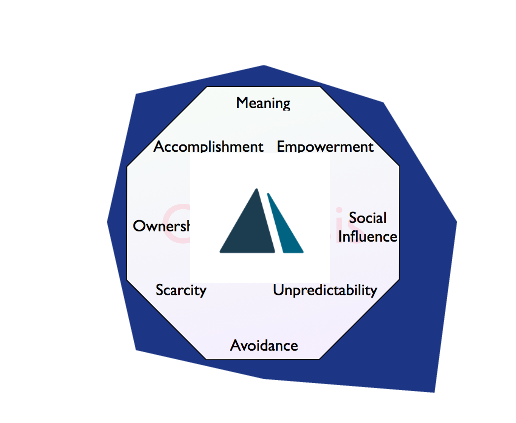
\includegraphics[width=400px, scale=1]{figuras/fasedescoberta}
    \caption{Fase Descoberta}
    \label{fig:fasedescoberta}
\end{figure}

No momento de uma propaganda este lado do \textit{framework} pode gerar uma
extrema curiosidade no usuário, o que fará com que ele fique motivado a procurar
e entender mais sobre o que está sendo anunciado.

Isto pode ser extremamente importante para conseguir capturar novos usuários.

Na segunda fase, em que o usuário vai conhecer sobre o produto, pode ser visto
na figura \ref{fig:fasereconhecimento} que as fases relativas a desenvolvimento próprio e realização de si mesmo
são bem mais presentes, bem como o empoderamento e \textit{feedback}, que serão
responsáveis por fazer com que o usuário sinta que consegue e é capaz
de realizar as atividades que são designadas.

\begin{figure}[h]
    \centering
    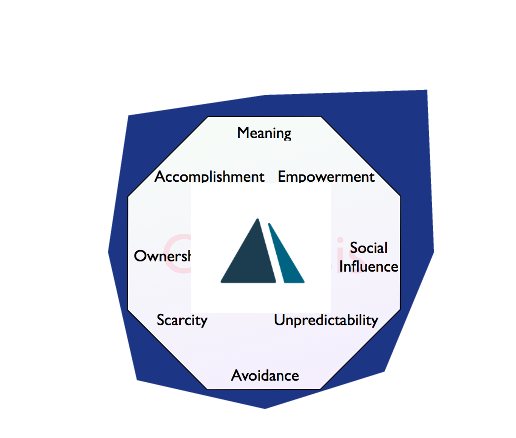
\includegraphics[width=400px, scale=1]{figuras/fasereconhecimento}
    \caption{Fase Reconhecimento}
    \label{fig:fasereconhecimento}
\end{figure}

Este ponto pode ser aplicado, pois o usuário irá se sentir realizado e inteligente
ao observar seu desenvolvimento próprio elevado. Isto irá gerar um prazer em fazê-lo
sentir o quanto pode ser bom em realizar as tarefas que a ele estão sendo designadas
no início do procedimento.

Na terceira fase é possível verificar que três motivações básicas são muito presentes,
assim como pode ser conferido na Figura \ref{fig:faseconstrucao}:



\begin{itemize}
    \item Motivação Básica Cinco: Influência e Dinâmica Social;
    \item Motivação Básica Seis: Escassez e Impaciência.
    \item Motivação Básica Sete: Curiosidade e Imprevisibilidade.
\end{itemize}

\begin{figure}[h]
    \centering
    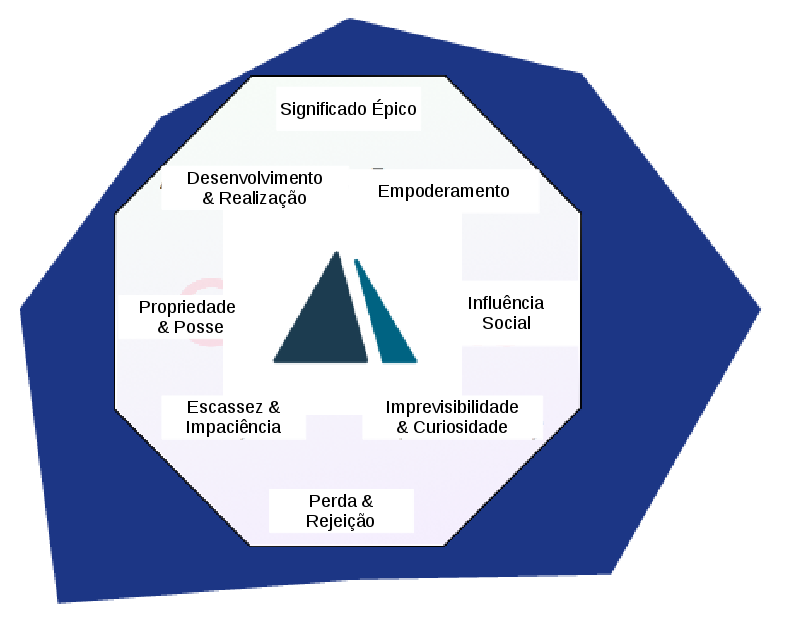
\includegraphics[width=300px, scale=1]{figuras/faseconstrucao}
    \caption{Fase Construção}
    \label{fig:faseconstrucao}
\end{figure}


Para a Motivação Básica Cinco, isto deixa o usuário motivado ao utilizar o produto
por sentir que está exercendo uma alta influência social, que está envolvido em
uma dinâmica social que faz influência em outras pessoas.

Isto faz com que o usuário fique motivado a continuar engajado no processo, pois,
este estará conseguindo perceber o quanto está sendo participativo no meio social
e que o produto está sendo proveitoso por fazê-lo se sentir socialmente influente
e participativo.


A segunda motivação básica vizualizada nesta fase, Escassez e Impaciência, acontece
pois é possível verificar que o usuário fique motivado a executar determinadas
tarefas baseado neste sentimento.

Esta o deixará preocupado com a questão de não cumprir corretamente os objetivos.
Esta fase é responsável por fazê-lo se sentir em um meio escasso caso não execute
os objetivos propostos.

Isto vai motivar o usuário e vai fazer com que faça o necessário para que não
sinta estes sentimentos.

A última fase, fim de jogo, também tem sua motivação básica predominante que
a guia. Esta é guiada pela Motivação Básica Oito: Perca e evitação, que pode
ser conferida na Figura \ref{fig:fasefimdejogo}.

\begin{figure}[h]
    \centering
    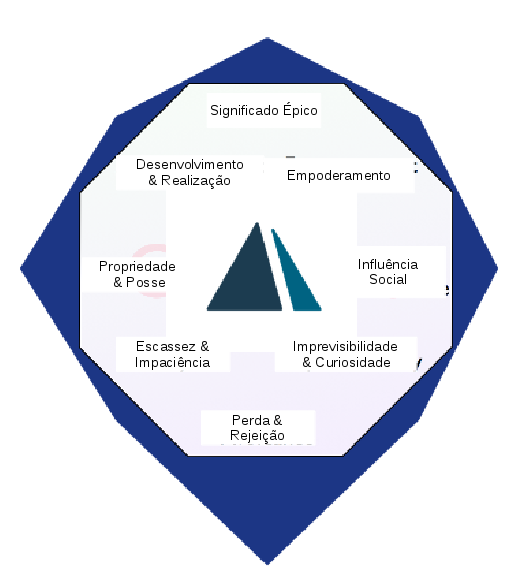
\includegraphics[width=300px, scale=1]{figuras/fasefimdejogo}
    \caption{Fase Fim de Jogo}
    \label{fig:fasefimdejogo}
\end{figure}

Esta irá gerar um sentimento que faz o usuário se sentir mal. Este sentimento
envolve o fato de que o usuário pode perder todo o processo que foi executado.


Este é um sentimento ruim. Sentimento qual o usuário não deseja sentir. Para tanto
ele se esforçará a fim de não presenciar as experiências que são submetidas.

Como pode ser visto, estes procedimentos de cada fase são extremamente aplicáveis
e úteis para que o usuário tenha várias experiências ao longo do ciclo de vida do
produto. O que propiciará uma experiência muito mais agradável.

Dessa forma, serão desenhados quatro \textit{frameworks} diferentes para a Rede Social About.
Uma para cada fase diferente do produto, onde serão estudadas separadamente para
aplicá-las e possibilitar uma boa experiência para o usuário.

\subsection{\textit{Octalysis} \textit{Strategy} \textit{Dashboard}}
\label{sec:octalysisdashborad}
Para este desenvolvimento, serão utilizados os procedimentos sistematizados adotados
pelo \textit{Octalysis} \textit{Strategy} \textit{Dashboard}(OSD), auxiliando assim no processo sistemático para
a execução do projeto. 

Assim, de acordo com a metodologia, as fases executadas serão regidas de acordo com a
figura a seguir.  Além disso, serão descritos subcapítulos, que retratarão o papel e a 
utilidade de cada componente dentro do processo de desenvolvimento.


 \begin{figure}[h]
     \centering

     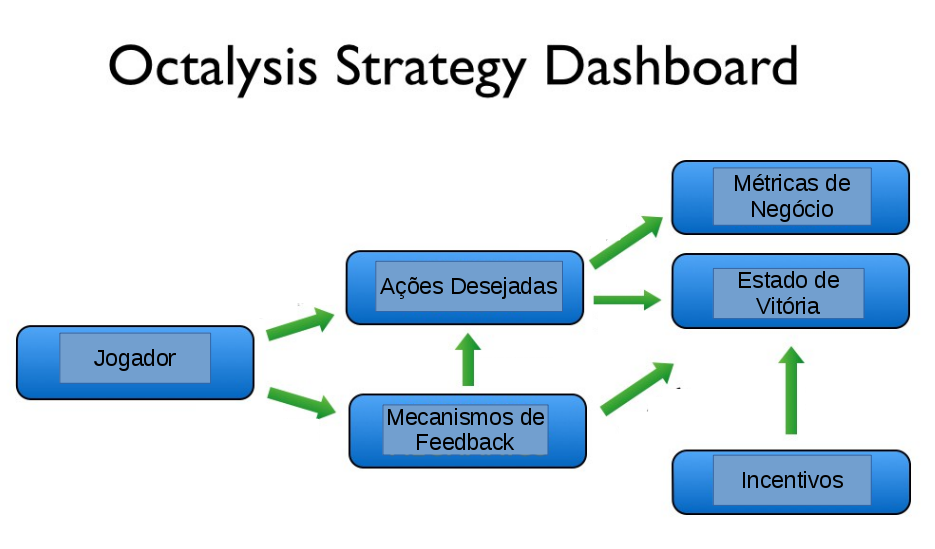
\includegraphics[width=450px, scale=1]{figuras/dashboard}
     \caption{\textit{Octalysis} \textit{Strategy} \textit{Dashboard}}

     \label{fig:dashboard}
 \end{figure}

\subsubsection{Métricas de Negócio}
\label{sub:business_metrics}
As métricas de negócio, em português, são termos quantitativos que podem ser utilizados
para ter um número palpável sobre como está um determinado ponto do projeto de gamificação
que teve como o objetivo de ser atacado.

Essas métricas, irão auxiliar a verificarmos o quanto a aplicação da gamificação foi 
eficaz ou não dentro de um determinado objetivo.

As métricas de negócio que irão direcionar a aplicação da rede social about estão
descritos a seguir:

\begin{itemize}
    \item Aumentar o número de seguidores dos usuários prêmio;
    \item Aumentar o número de inscritos na rede social;
    \item Aumentar a quantidade de acessos diários;
    \item Aumentar os seguidores inscritos na rede sociai;
    \item Aumentar os usuários que compartilham conteúdos pelas redes sociais;
    \item Aumentar a quantidade de julgamentos em abouts;
    \item Aumentar a quantidade de abouts criados;
\end{itemize}

Estas métricas serão submetidas à Rede Social About antes da apresentação da
gamificação. E assim que determinada técnica for utilizada, será então executada uma
segunda medição, que propiciará analisar as diferenças entre os resultados obtidos.

\subsubsection{Definir Tipos de Usuário}
\label{sub:define_user_types}
Este ponto do \textit{dashboard}, para definir os tipos dos usuários, irá
definir quais são os tipos de usuários que serão almejados e trabalhados, quando
falamos sobre gamificação.

Esta fase é um processo de definição de nicho sobre onde a gamificação vai atuar, quanto a
usuários, dentro da Rede Social About? Quais serão os passos utilizados para que este público
seja atingindo?

Alguns exemplos de tipos de usuário se encontram a seguir:

\begin{itemize}
    \item Companhias que desejam que seus trabalhadores atinjam determinadas métricas
        ao fim de cada mês;
    \item Educadores e políticos que querem utilizar conhecimento para criar impactos
        sociais;
    \item Indivíduos que são apaixonados por gamificação, games e desenvolvimento próprio.
\end{itemize}

Desta maneira, será possível realizar um projeto de gamificação focado ao definir o tipo
de usuário. Pois, a partir daí, será possível identificar quais caminhos são mais vantajosos
quanto a escolha das motivações básicas que serão utilizadas ao longo das quatro fases.

\subsubsection{Definir Ações Desejadas}
\label{sub:define_desired_actions}
A definição das ações desejadas são todas as iniciativas tomadas pelo usuário que o 
levam a caminhar para
o \textit{Win} \textit{Stade}(Estado de Vitória), seja ela em qual fase for. Sendo assim, a Rede Social
About terá alguns pontos que serão definidos como os desejados. Estes serão desenhados
até que o estado de vitória seja definido. Assim, para as quatro fases serão definidas
ações diferentes. Estas são as  ações que serão escolhidas e apresentadas
a seguir.

Ações na fase da descoberta:
\begin{itemize}
    \item Conhecer a Rede Social About;
    \item Clicar no link da Rede Social About;
    \item Conhecer as \textit{features} oferecidas pela Rede Social;
\end{itemize}


Ações na fase de reconhecimento do projeto: 
\begin{itemize}
    \item Executar o tutorial de uso da About;;
    \item Compartilhar a Rede Social About com os amigos;
    \item Adicionar foto e email na \textit{network};
    \item Permitir a inscrição na lista de email;
\end{itemize}

Já para a fase de construção do projeto, os seguintes pontos serão
abordados:

\begin{itemize}
    \item Fazer \textit{login} diariamente na \textit{network};
    \item Abrir semanalmente os emails enviados pela \textit{network};
    \item Compartilhar abouts com os amigos;
    \item Participar de grupos no \textit{Facebook} sobre a rede social about;
    \item Adquirir a versão prêmio da rede social about;
    \item Inscrever em grupos de discussão sobre a rede social about;
    \item Escrever mais de um about diariamente;
    \item Votar em mais de vinte abouts diários;
\end{itemize}

Por fim, na fase de fim de jogo, alguns exemplos de construção podem ser dados. Eles são os seguintes:
\begin{itemize}
    \item Se tornar contribuidor da Rede Social About;
    \item Fazer parte da equipe de desenvolvedores da About;
    \item Propor melhorias para a about;
    \item Tornar-se moderador dos abouts;
\end{itemize};

Estes pontos desejados ajudam e esclarecer como os objetivos podem ser alcançados. Elas 
definem um nível de granularidade maior.

\subsubsection{Definir Mecanismos de Feedback}
\label{sub:define_feedback_mechanics}
A definição de mecanismos de \textit{feedback} são extremamente importantes para a experiência 
do usuário
com a \textit{network}. Este é responsável por ilustrar e deixar bem claro para o usuário, como 
ele está prosseguindo no desenvolvimento do projeto.

Atualmente os usuários tem requirido \textit{feedbacks} constantes, em tempo real, para as suas 
ações
realizadas. Sendo assim, é necessário que existam esses gatilhos em vários pontos da
Rede Social About e que o usuário possa entender rapidamente.

A seguir estão os pontos  de como devem ser exclarecidos esses \textit{feedbacks} para o 
usuário:

\begin{itemize}
    \item \textit{Countdown} \textit{Timers};
    \item Verificação de qual era a melhor escolha;
    \item Barra de pontos de status;
    \item Certificados;
    \item Medalhas;
    \item Gráficos de desempenho;
\end{itemize}

Assim, com estes mecanismos definidos dessa maneira, é possível que o usuário verifique 
o quanto suas atividades estão sendo aproveitadas.

\subsubsection{Incentivos e Recompensas}
\label{sub:incentives_and_rewards}
O sistema de incentivos e recompensas fecham o ciclo do \textit{dashboard}, que fazem com que 
os usuários se sintam motivados a alcançar cada estado de vitória. Eles ajudam a indicar
o quanto ainda falta para que o estado seja almejado.

\begin{itemize}
    \item \textit{Status} \textit{Points};
    \item Símbolos de vitórias;
    \item Conhecer os desenvolvedores da about;
    \item Ter acesso a arquivos confidenciais;
    \item Descontos nos produtos;
\end{itemize}

\section{Planejamento do Projeto}
\label{sub:planejamento_do_projeto}
O procedimento de aplicação do projeto de gamificação conterá algumas fases
e etapas para serem executadas. Estas etapas estão ilustradas nas macroatividades 
descritas no processo que foi desenhado para guiar o desenvolvimento
do projeto.

A imagem a seguir representa o processo que será utilizado.

\begin{figure}[h]
    \centering
    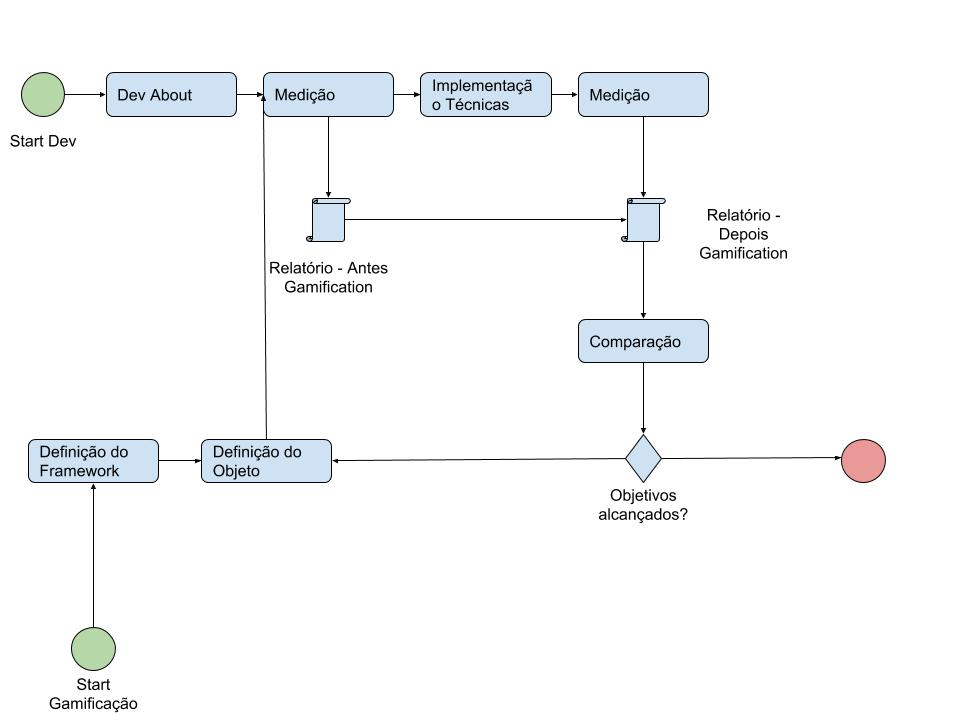
\includegraphics[width=450px, scale=1]{figuras/mainprocess}
    \caption{Processo Principal}
    \label{fig:mainprocess}
\end{figure}

\subsection{Início do Processo}
\label{sub:initialprocess}
Como pode ser observado na figura \ref{fig:mainprocess}, existem dois pontos
de início independentes no desenvolvimento do projeto. Um deles, se trata do
\textit{Start} \textit{Dev}, sendo que o outro é o \textit{Start} gamifição. O primeiro retrata sobre
o início do desenvolvimento, que dará início a aplicação da about \textit{network}
como produto. Nesta serão utilizadas as técnicas de desenvolvimento de \textit{software}
e técnicas de codificação a parte, até que esta esteja disponível para receber
usuários e esteja passível de executar uma medição. Já o segundo ponto de início
retrata o começo do desenvolvimento do \textit{framework} de gamificação que será utilizado,
bem como definição de quais serão os pontos abordados do processo de gamificação.
Estas duas atividades podem trabalhar paralelamente e não tem a necessidade de
serem iniciadas ao mesmo tempo. Desta forma, são criados esses dois pontos de
entrada do projeto.

\subsection{Desenvolvimento About}
\label{sub:Desenvolvimentoabout}
Em seguida, é possível observar a macroatividade \textit{Dev} \textit{About}, que é responsável
por tornar prática a ideia da Rede Social About. Nela serão aplicadas as
regras de desenvolvimento para que seja possível implementar todos os
requisitos propostos.

Este protótipo deverá ser operacional, a modo com que os usuários consigam
utilizá-lo e seja possível obter algumas estatísticas sobre uso que comprovem
de fato quais são os índices de utilização do site pelo usuário quantativamente.

Logo a frente existe a atividade de mediação, onde a partir desta serão retirados
os resultados de uso e estatísticas que consigam interpretar variáveis da gamificação
dentro do produto de \textit{software}. 

\subsection{Medição}
\label{sub:medicao}
Pode ser observado que existem duas atividades de medição. A primeira se dá
antes da implementação do \textit{framework}  e das técnicas de gamificação na about.

Já a segunda tem o objetivo de retratar o quanto os índices se alteraram após
a aplicação do \textit{framework} na rede social about.

Estas atividades de medição irão gerar relatórios, que armazenarão os resultados
e, posteriormente, serão comparadas para verificar as diferenças entre ambos.

\subsection{Definição do \textit{Framework}}
\label{sub:definicaoframework}
A macroatividade de definição do \textit{framework} será responsável por fazer um grande
trabalho, desde um estudo avaliativo do procedimento para a verificação de como
devem ser aplicadas corretamente as técnicas de gamificação até bem como o desenho
do \textit{framework} que será utilizado e aplicado na Rede Social About.

Ao final desta atividade, será possível obter insumos necessários para a definição
dos objetivos de gamificação, os quais serão desenhados e aplicados a fim
de nortear sobre quais rumos o projeto tomará.

É exatamente neste ponto que o projeto de gamificação e o desenvolvimento do produto
se encontram. Eles irão juntos verificar como estão as medidas de gamificação, para
então, a partir daí, ser possível aplicar as técnicas implementadas.

\subsection{Implementação das Técnicas}
\label{sub:implematationtechnics}
A macroatividade de Implementação das Técnicas será utilizada para que, a partir
dos objetivos definidos anteriormente, seja possível construir o produto de \textit{software}
de fato. Esta será responsável por tornar prática
cada técnica que foi definida.

Bem como quando forem definidas cada técnica, na prática, esta macroatividade
será a utilizada para codificar e tornar apresentável para o usuário o que
foi definido no contexto da gamificação.

\subsection{Comparação}
\label{sub:Comparacao}
Em seguida é possível observar a macroatividade de Comparação, que será
responsável por averiguar quais os níveis de diferença entre as medições que
antecedem e procedem a implementação das técnicas. Estes dados serão recolhidos a
partir dos relatórios obtidos com os resultados das medições.

\subsection{Finalização do Processo}
\label{sub:finalprocess}
Assim que a comparação for executada, já será possível escolher se os objetivos
foram alcançados ou não. Com base nessa resposta, a atividade de escolha irá
identificar se é necessário refazer o processo e voltar para a refazer a fase
de definição de objetivo ou se este pode ser finalizado.

Caso na atividade de decisão seja verificado que não há a necessidade de
redefinição, o ciclo irá se repetir até que o resultado seja satisfatório.

\subsection{Cronograma}
\label{sub:cronograma}
Para auxiliar na execução das tarefas, foi elaborado um cronograma
das macro atividades que serão elaboradas ao longo de desenvolvimento.

A seguir, estão representadas as datas das entregas, bem como o diagrama
de gant destas.

\begin{figure}[h]
    \centering
    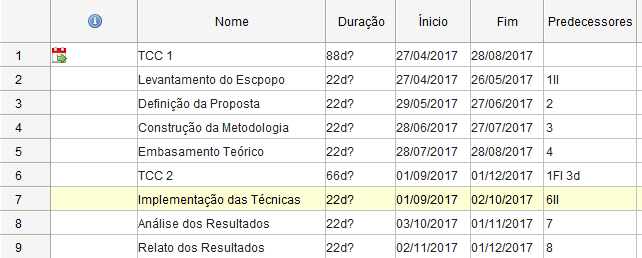
\includegraphics[width=400px, scale=1]{figuras/cronogramadatas}
    \caption{Cronograma por Datas}
    \label{fig:cronogramadatas}
\end{figure}

\begin{figure}[h]
    \centering
    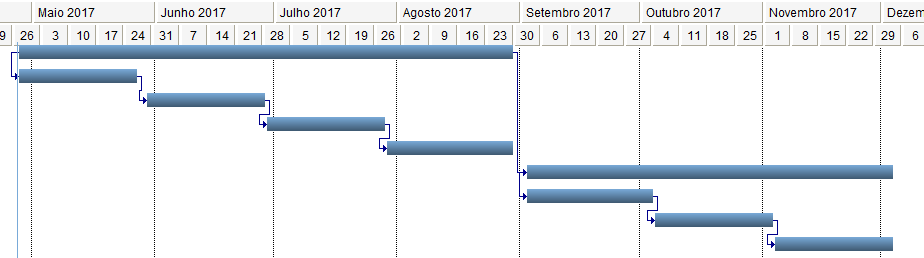
\includegraphics[width=400px, scale=1]{figuras/cronogramabarras}
    \caption{Cronograma por Barras}
    \label{fig:cronogramabarras}
\end{figure}
